%!TEX root = ../thesis.tex
%*******************************************************************************
%****************************** Third Chapter **********************************
%*******************************************************************************
\chapter{Experiments and Results}
\label{ch3}
% **************************** Define Graphics Path **************************
\ifpdf
    \graphicspath{{Chapter3/Figs/Raster/}{Chapter3/Figs/PDF/}{Chapter3/Figs/}}
\else
    \graphicspath{{Chapter3/Figs/Vector/}{Chapter3/Figs/}}
\fi
%

This section details and presents the empirical evaluations conducted utilizing the methodologies delineated in the preceding chapter. 
The analysis commences with a formal characterization of the fundamental objective: quantifying the cultural competency of ML models under conditions of significant data sparsity and under-representation.
Subsection sections provide an assessment of the cultural competence of baseline ML models under varying degrees of cultural under-representation.
Finally, we provide a comprehensive exposition of the experimental results obtained for the MTL architecture..

\section{Evaluating Machine Learning Cultural Competence Under Data Scarcity}
\label{ch3:sec:exp_standard_ml}
%
The No-Free-Lunch theorem~\citep{wolpert1996lack} posits that no single learning algorithm is universally superior across all possible data distributions.
Consequently, identifying the optimal architecture for a specific application necessitates an empirical comparison of multiple algorithmic frameworks, as an optimal choice cannot be determined a priori.

Adhering to this principle, the present study evaluates two of the most robust and empirically successful algorithms for binary classification—specifically, SVM and Deep Neural Networks—which have consistently demonstrated state-of-the-art performance across diverse tabular and high-dimensional benchmarks~\citep{fernandez2014we,wainberg2016random,shu2021zoo}.

The first candidate originates from the domain of shallow learning architectures: Support Vector Machines (SVM)~\citep{shalev2014understanding}, utilizing both Linear and Gaussian (RBF) kernels~\citep{6790031}. 
In this framework, the input space is defined as $\mathcal{X} = \mathbb{R}^d$, where $d$ represents the vectorized pixel intensities of the images converted to grayscale.
To ensure structural homogeneity across the dataset, we evaluated several preprocessing techniques, such as zero-padding and spatial rescaling. We ultimately opted to rescale all instances to a uniform resolution ($d = 35 \times 35$) via area interpolation (inter-area) using the OpenCV library.For the Linear SVM (LSVM), the mapping $\varphi$ in Eq.~\eqref{ch2:eq:generalproblem} is the identity function. 
The optimization objective incorporates the Hinge loss function, $\max(0, 1 - y f(x))$, and an $L_2$ regularizer $\lambda \| \mathbf{w} \|^2_2$, where $\lambda$ is a hyperparameter determined through a formal model selection phase. 
Conversely, for the Gaussian SVM (GSVM), the configuration remains identical to the LSVM, with the exception that $\varphi$ is implicitly induced by a Gaussian kernel. 
This kernel is characterized by the bandwidth parameter $\sigma^2$ (variance), which is similarly optimized during the model selection procedure.

The second algorithmic framework is denoted as RESNET. 
This approach utilizes a pre-trained ResNet architecture~\citep{He_2016_CVPR} as a feature extractor, followed by a linear classification head employing a Sigmoid activation function. 
The model is optimized via the Binary Cross-Entropy (BCE) loss function and the Adam optimizer.
For the RESNET configuration, the input space is defined as $\mathcal{X} = \mathbb{R}^{3 \times H \times W}$, where the spatial dimensions are set to $H = W = 120$ for the LAMP dataset and $H = W = 200$ for the CARPET dataset. 
To facilitate convergence, we implement a dynamic learning rate scheduler that decays the learning rate upon detecting an accuracy plateau~\citep{goodfellow2016deep}.

The training procedure is partitioned into two distinct phases. 
In the initial phase, the optimization is restricted to the weights of the classification head, effectively utilizing the backbone as a fixed feature extractor. 
However, empirical analysis of the datasets revealed that the feature representations learned on ImageNet are insufficiently aligned with the nuances of the current problem domain, necessitating a refinement of the internal parameters.
Consequently, a fine-tuning phase is executed, wherein the entire network architecture is optimized using a significantly reduced learning rate, $l_{r_{fn}}$. 
During the Model Selection phase, we perform a grid search over the primary learning rate $l_r$ and the epoch count $n_e$, while the fine-tuning rate is held constant at $l_{r_{fn}} = 10^{-5}$.
A comprehensive summary of the model architectures and the associated hyperparameter ranges utilized for model selection and error estimation is detailed in Table~\ref{ch3:tab:hyper}.
%
\begin{table}
\footnotesize
\centering
\setlength{\tabcolsep}{0.1cm}
\renewcommand{\arraystretch}{1.5}
\centering
\begin{tabular}{c|c|c}
\toprule
\textbf{Model} & \textbf{Hyper.} & \textbf{Ranges/Setting} \\
\midrule
\multicolumn{3}{c}{\textbf{ML Algorithms (Section~\ref{ch3:sec:exp_standard_ml})}}\\
\midrule
\multirow{3}{*}{LSVM} & $n_r$ & $10$ \\
\hhline{~--}
& $|\mathcal{L}^r|, |\mathcal{V}^r|, |\mathcal{T}^r|$& $80\%, 10\% 10\%$ \\
\hhline{~--}
& $\lambda$ & $10^{-4.0},10^{-3.8}, \cdots, 10^{-3.0}$\\
\midrule
\multirow{5}{*}{GSVM} & $n_r$ & $10$ \\
\hhline{~--}
& $|\mathcal{L}^r|, |\mathcal{V}^r|, |\mathcal{T}^r|$& $80\%, 10\% 10\%$ \\
\hhline{~--}
& $\lambda$ & $10^{-4.0},10^{-3.8}, \cdots, 10^{-3.0}$\\
\hhline{~--}
& $\sigma^2$ & $10^{-4.0},10^{-3.8}, \cdots, 10^{-3.0}$\\
\midrule
\multirow{4}{*}{RESNET} & $n_r$ & $10$ \\
\hhline{~--}
& $|\mathcal{L}^r|, |\mathcal{V}^r|, |\mathcal{T}^r|$& $70\%, 20\% 10\%$ \\
\hhline{~--}
& $l_r$ & $.0001, .0005, \cdots, .1$\\
\hhline{~--}
& $n_e$ & $4,6, \cdots, 30$\\
\midrule
\multicolumn{3}{c}{\textbf{Addition of Cultural Competence (Section~\ref{ch2:sec:makeMLcultcomp})}}\\
\midrule
\multicolumn{3}{c}{Same as above plus}\\
* & $\gamma$ & $10^{-2.0},10^{-1.84}, \cdots, 10^{+2.0}$\\
\bottomrule
\end{tabular}
\caption{ML algorithms and related hyperparameters range and settings.}
\label{ch3:tab:hyper}
\end{table}
%
To rigorously evaluate the cultural (in)competence of the models, we conducted a systematic analysis of the effects of cultural under-representation within the training distribution.
Specifically, we established a single dominant culture within the learning set and modulated the representation density of the remaining cultures via a parameter $p_u$, representing the percentage of available data for each non-dominant group. For instance, utilizing the LAMP dataset, we evaluated a baseline configuration comprising exclusively Chinese lamps. 
We subsequently introduced samples from French and Turkish cultural contexts at varying concentrations, such as $p_u = 10\%$.
The empirical observations were recorded across a spectrum of under-representation levels, specifically $p_u \in \{0\%, 5\%, 10\%\}$.
%
\section{Mitigation Strategies}
%\label{ch3:sec:exp_mitigation}
The first proposed mitigation strategy is integrated into the RESNET framework, which was identified as the superior architecture based on the empirical results presented in Section~\ref{ch3:sec:exp_standard_ml}. 
This evaluation focuses on both the LAMP and CARPET datasets across the under-representation levels $p_u \in \{5\%, 10\%\}$. 
Note that the case $p_u = 0\%$ is excluded from this analysis, consistent with the theoretical constraints of MTL delineated in Section~\ref{ch2:sec:CCML}, which require at least a minimal presence of cultural labels for the auxiliary task.
The expanded hypothesis space $\mathcal{H}$, which incorporates the additional regularization parameter $\gamma$ governing the MTL task-weighting, is detailed in Table~\ref{ch3:tab:hyper}.
%

\section{Baseline Evaluation of Cultural Incompetence}

For the LAMP dataset, we conducted a comparative performance evaluation of the LSVM, GSVM, and RESNET architectures. 
In contrast, the analysis of the CARPET dataset was restricted to the RESNET framework due to the heightened complexity of the classification task; preliminary empirical assessments indicated that the linear and kernel-based SVMs (LSVM and GSVM) failed to achieve acceptable accuracy thresholds.

The comprehensive results regarding cultural competence and the baseline performance of these standard ML algorithms for both the LAMP and CARPET use cases are detailed in Tables~\ref{ch3:tab:ris:ml:lamp} and \ref{ch3:tab:ris:ml:carpet}, with corresponding visual trends illustrated in Figures~\ref{ch3:fig:ris:ml:lamp} and \ref{ch3:fig:ris:ml:carpet}.

Table~\ref{ch3:tab:ris:ml:lamp} delineates the test set error rates for the LAMP dataset across each cultural category—specifically $\text{ERR}^{\text{Chin.}}$, $\text{ERR}^{\text{Fren}}$, and $\text{ERR}^{\text{Turk.}}$—alongside the CIC for the LSVM, GSVM, and RESNET architectures. 
These metrics are reported for every permutation of majority culture and minority representation level ($p_u$).
As a representative case, consider the RESNET performance when the majority culture is Fren and the minority representation is $p_u=0\%$. In this configuration, the error for the dominant class ($\text{ERR}^{\text{Fren}}$) is $34.6\%$, which is significantly lower than the error rates observed for the Chin. and Turk. categories. 
However, empirical trends indicate that as $p_u$ increases, the error rate for the majority culture typically rises, whereas the error rates for the minority cultures and the overall CIC exhibit a downward trajectory, suggesting a more balanced feature representation.

Table~\ref{ch3:tab:ris:ml:carpet} serves as the counterpart to Table~\ref{ch3:tab:ris:ml:lamp} for the CARPET dataset, where experimental evaluations are restricted to the RESNET architecture.
To enhance interpretability and provide a comprehensive visualization, Figure~\ref{ch3:fig:ris:ml:lamp} illustrates the data from Table~\ref{ch3:tab:ris:ml:lamp} in a graphical format. 
The horizontal axis represents the test error (ERR), while the vertical axis denotes the CIC as the minority representation $p_u$ varies. 
The trajectory of $p_u$ is indicated by directional arrows, which signify the evolution of performance as the minority data percentage increases. 
Within each plot, which corresponds to a specific majority culture, the arrow's color identifies the culture for which the ERR is computed, while the line style (solid, dashed, or dotted) distinguishes between the different algorithms employed.

Figure~\ref{ch3:fig:ris:ml:carpet} serves as the counterpart to Figure~\ref{ch3:fig:ris:ml:lamp} for the CARPET dataset, presenting the results obtained exclusively from the RESNET architecture.
%
\begin{table}
\footnotesize
\centering
\setlength{\tabcolsep}{0.1cm}
\renewcommand{\arraystretch}{1.1}
\begin{tabular}{c|c|c|c|c|c}
\toprule
\textbf{Algorithm} & \textbf{Majority} & \textbf{ERR$^{\text{Chin.}}$}
& \textbf{ERR$^{\text{Fren}}$}
& \textbf{ERR$^{\text{Turk.}}$} 
& \textbf{CIC} \\
\midrule
\multicolumn{1}{c}{\multirow{12}{*}{LSVM}} & \multicolumn{5}{c}{$p_u = 0\%$}\\
\hhline{~-----}
& Chin. & $33.1\% $ & $40.7\% $ & $44.4\% $ & $6.3\% $ \\
& Fren & $42.6\% $ & $34.6\% $ & $50.3\% $ & $7.9\% $ \\
& Turk. & $44.2\% $ & $45.9\% $ & $23.4\% $ & $14.4\% $ \\
\hhline{~-----}
\multicolumn{1}{c}{} & \multicolumn{5}{c}{$p_u = 5\%$}\\
\hhline{~-----}
& Chin. & $34.4\% $ & $38.3\% $ & $44.8\% $ & $4.7\% $ \\
& Fren & $40.9\% $ & $34.9\% $ & $46.9\% $ & $6.0\% $ \\
& Turk. & $42.4\% $ & $44.7\% $ & $24.8\% $ & $12.5\% $ \\
\hhline{~-----}
\multicolumn{1}{c}{} & \multicolumn{5}{c}{$p_u = 10\%$}\\
\hhline{~-----}
& Chin. & $35.1\% $ & $38.2\% $ & $43.7\% $ & $3.9\% $ \\
& Fren & $40.5\% $ & $35.2\% $ & $44.7\% $ & $5.0\% $ \\
& Turk. & $41.0\% $ & $44.4\% $ & $25.4\% $ & $11.5\% $ \\
\midrule
\multicolumn{1}{c}{\multirow{12}{*}{GSVM}} & \multicolumn{5}{c}{$p_u = 0\%$}\\
\hhline{~-----}
& Chin. & $27.0\% $ & $37.1\% $ & $43.5\% $ & $8.8\% $ \\
& Fren & $38.4\% $ & $33.7\% $ & $53.4\% $ & $8.1\% $ \\
& Turk. & $53.9\% $ & $49.7\% $ & $10.5\% $ & $27.5\% $ \\
\hhline{~-----}
\multicolumn{1}{c}{} & \multicolumn{5}{c}{$p_u = 5\%$}\\
\hhline{~-----}
& Chin. & $26.7\% $ & $34.0\% $ & $35.7\% $ & $5.4\% $ \\
& Fren & $36.8\% $ & $ 33.2\% $ & $36.2\% $ & $2.9\% $ \\
& Turk. & $41.6\% $ & $43.5\% $ & $10.9\% $ & $21.1\% $ \\
\hhline{~-----}
\multicolumn{1}{c}{} & \multicolumn{5}{c}{$p_u = 10\%$}\\
\hhline{~-----}
& Chin. & $28.0\% $ & $32.7\% $ & $26.0\% $ & $3.1\% $ \\
& Fren & $34.7\% $ & $32.1\% $ & $27.0\% $ & $4.2\% $ \\
& Turk. & $37.9\% $ & $39.1\% $ & $10.9\% $ & $18.4\% $ \\
\midrule
\multicolumn{1}{c}{\multirow{12}{*}{RESNET}} & \multicolumn{5}{c}{$p_u = 0\%$}\\
\hhline{~-----}
& Chin. & $15.2\% $ & $25.4\% $ & $46.4\% $ & $13.8\% $ \\
& Fren & $23.3\% $ & $10.6\% $ & $49.6\% $ & $17.3\% $ \\
& Turk. & $38.7\% $ & $44.3\% $ & $14.1\%$ & $18.6\% $ \\
\hhline{~-----}
\multicolumn{1}{c}{} & \multicolumn{5}{c}{$p_u = 5\%$}\\
\hhline{~-----}
& Chin. & $13.0\% $ & $21.5\% $ & $31.5\% $ & $9.0\% $ \\
& Fren & $20.9\% $ & $15.2\% $ & $33.3\% $ & $7.9\% $ \\
& Turk. & $27.9\% $ & $27.1\% $ & $12.6\% $ & $9.9\% $ \\
\hhline{~-----}
\multicolumn{1}{c}{} & \multicolumn{5}{c}{$p_u = 10\%$} \\
\hhline{~-----}
& Chin. & $11.2\%$ & $16.9\%$ & $23.3\%$ & $6.0\%$ \\
& Fren & $18.8\%$ & $11.6\%$ & $26.1\%$ & $7.2\%$ \\
& Turk. & $20.2\%$ & $22.6\%$ & $13.1\%$ & $5.5\%$ \\
\bottomrule
\end{tabular}
\caption{LAMP dataset: For each algorithm (LSVM, GSVM, and RESNET), for each combination of majority culture and $p_u$ (percentage of minority culture) in the training set, and for each possible combination of cultures (Chin., Fren, and Turk.), the error on the test set for each culture (ERR$^\text{Chin.}$, ERR$^\text{Fren}$, and ERR$^\text{Turk.}$) and the CIC are reported.}
\label{ch3:tab:ris:ml:lamp}
\end{table}
%
%
\begin{table}
\footnotesize
\centering
\setlength{\tabcolsep}{0.1cm}
\renewcommand{\arraystretch}{1.55}
\begin{tabular}{c|c|c|c|c|c}
\toprule
\textbf{Algorithm} & \textbf{Majority} & \textbf{ERR$^{\text{Ind.}}$}
& \textbf{ERR$^{\text{Japan.}}$}
& \textbf{ERR$^{\text{Scand.}}$} 
& \textbf{CIC} \\
\midrule
\multicolumn{1}{c}{\multirow{12}{*}{RESNET}} & \multicolumn{5}{c}{$p_u = 0\%$}\\
\hhline{~-----}
& Ind. & $24.1\% $ & $33.3\% $ & $44.1\% $ & $9.8\% $ \\
& Japan. & $36.7\% $ & $22.3\% $ & $50.8\% $ & $14.3\% $ \\
& Scand. & $41.3\% $ & $52.6\% $ & $35.7\% $ & $7.9\% $ \\
\hhline{~-----}
\multicolumn{1}{c}{} & \multicolumn{5}{c}{$p_u = 5\%$}\\
\hhline{~-----}
& Ind. & $25.4\% $ & $30.7\% $ & $42.3\% $ & $7.5\% $ \\
& Japan. & $33.4\% $ & $17.8\% $ & $50.1\% $ & $16.0\% $ \\
& Scand. & $37.5\% $ & $41.5\% $ & $36.3\% $ & $3.5\% $ \\
\hhline{~-----}
\multicolumn{1}{c}{} & \multicolumn{5}{c}{$p_u = 10\%$}\\
\hhline{~-----}
& Ind. & $26.1\% $ & $30.4\% $ & $44.8\% $ & $7.7\% $ \\
& Japan. & $33.2\% $ & $20.6\% $ & $48.7\% $ & $13.6\% $ \\
& Scand. & $33.7\% $ & $34.4\% $ & $35.2\% $ & $2.6\% $ \\
\midrule
\end{tabular}
\caption{CARPET dataset: For the RESNET algorithm, for each combination of majority culture and $p_u$ (percentage of minority culture) in the training set, and for each possible combination of cultures (Ind., Japan., and Scand.), the error on the test set for each culture (ERR$^\text{Ind.}$, ERR$^\text{Japan.}$, and ERR$^\text{Scand.}$) and the CIC are reported.}
\label{ch3:tab:ris:ml:carpet}
\end{table}
%
%
\begin{figure}
\centering
\begin{subfigure}[b]{0.325\columnwidth}
\centering
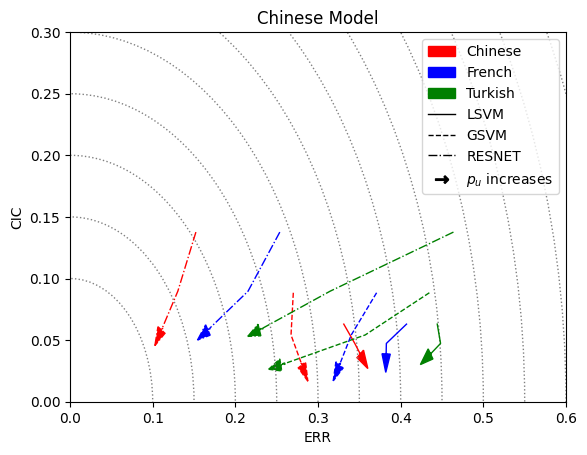
\includegraphics[width=\columnwidth]{Chapter3/FirstPaperFigures/analisi_chinese.png}
\caption{Majority - Chin.}
\end{subfigure}
\begin{subfigure}[b]{.325\columnwidth}
\centering
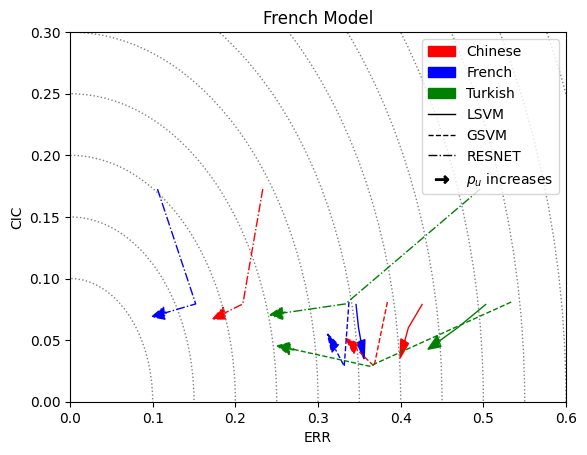
\includegraphics[width=\columnwidth]{Chapter3/FirstPaperFigures/analisi_french.png}
\caption{Majority - Fren}
\end{subfigure}
\begin{subfigure}[b]{.325\columnwidth}
\centering
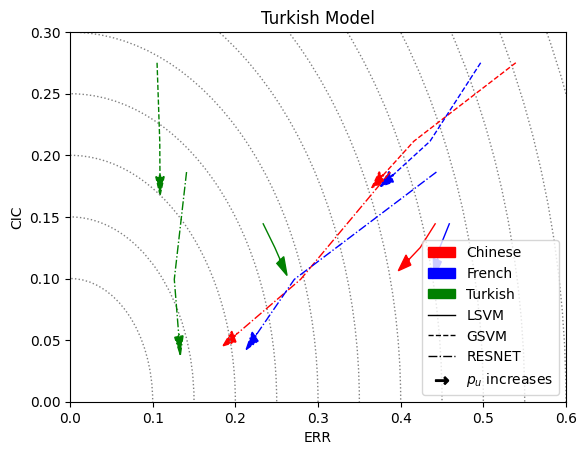
\includegraphics[width=\columnwidth]{Chapter3/FirstPaperFigures/analisi_turkish.png}
\caption{Majority - Turk.}
\end{subfigure} 
\caption{LAMP dataset: graphical representation of Table~\ref{ch3:tab:ris:ml:lamp}. 
x-axis reports the average error on all cultures (ERR) while on the y-axis the CIC varying $p_u$ (arrow indicates the direction of increase of $p_u$) for each algorithm (LSVM, GSVM and RESNET) and for each combination of majority culture and $p_u$ (percentage of minority culture) in the training set and for each possible combination of the cultures (Chin., Fren, and Turk.).}
\label{ch3:fig:ris:ml:lamp}
\end{figure}
%
%
\begin{figure}
\centering
\begin{subfigure}[b]{.325\columnwidth}
\centering
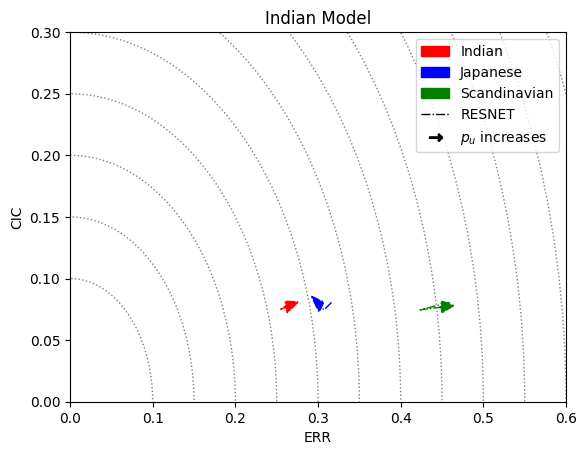
\includegraphics[width=\columnwidth]{Chapter3/FirstPaperFigures/analisi_indian.png}
\caption{Majority - Ind.}
\end{subfigure}
\begin{subfigure}[b]{.325\columnwidth}
\centering
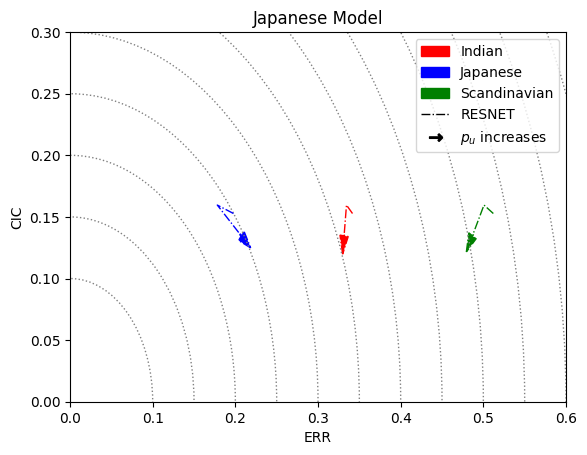
\includegraphics[width=\columnwidth]{Chapter3/FirstPaperFigures/analisi_japanese.png}
\caption{Majority - Japan.}
\end{subfigure}
\begin{subfigure}[b]{.325\columnwidth}
\centering
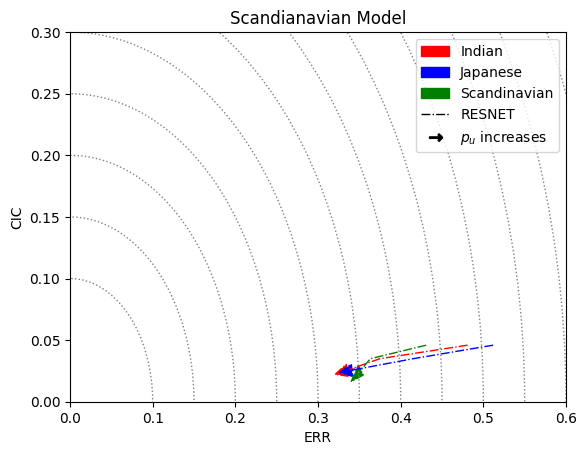
\includegraphics[width=\columnwidth]{Chapter3/FirstPaperFigures/analisi_scandinavian.png}
\caption{Majority - Scand.}
\end{subfigure} 
\caption{CARPET dataset: A graphical representation of Table~\ref{ch3:tab:ris:ml:carpet}. The x-axis shows the average error across all cultures (ERR), while the y-axis represents the CIC varying with $p_u$ (the arrow indicates the direction of increase of $p_u$). This is for the RESNET algorithm and for each combination of majority culture and $p_u$ (percentage of minority culture) in the training set, as well as for each possible combination of the cultures (Ind., Japan., and Scand.).}
\label{ch3:fig:ris:ml:carpet}
\end{figure}
%
\section{Multi-Task-Learning-Inspired Mitigation Strategy}
\label{sec:exp_mitigation:res}
The proposed mitigation framework is applied to the RESNET architecture—identified as the optimal model based on the empirical results delineated in the previous chapter—across both the LAMP and CARPET datasets. 
Evaluations are conducted using minority representation levels $p_u \in \{5\%, 10\%\}$, excluding the $p_u = 0\%$ configuration in accordance with the theoretical constraints established in Section~\ref{ch2:sec:CCML}.
The performance metrics for the MTL interventions are detailed in Tables~\ref{ch3:tab:ris:mtl:lamp} and~\ref{ch3:tab:ris:mtl:carpet}, and further elucidated through the graphical representations in Figures~\ref{ch3:fig:ris:mtl:lamp} and~\ref{ch3:fig:ris:mtl:carpet}.

Table~\ref{ch3:tab:ris:mtl:lamp} details the performance of the mitigated RESNET architecture on the LAMP dataset across each permutation of majority culture and minority representation levels ($p_u \in \{5\%, 10\%\}$). 
The table enumerates the results for varying threshold values $\tau \in \{0, 0.05, 0.1\}$ across all cultural combinations (Chin., Fren, and Turk.).
Specifically, it reports the optimal task-weighting parameter identified during model selection, denoted as $\gamma^*$, the class-specific test error rates ($\text{ERR}^{\text{Chin.}}$, $\text{ERR}^{\text{Fren}}$, and $\text{ERR}^{\text{Turk.}}$), and the resulting CIC. 
Furthermore, to quantify the efficacy of the MTL approach, we provide the percentage improvement ($\%\text{Imp.}$) relative to the non-mitigated baseline configurations established in Section~\ref{ch3:sec:exp_standard_ml} (see Table~\ref{ch3:tab:ris:ml:lamp}).

Table~\ref{ch3:tab:ris:mtl:carpet} provides analogous performance metrics for the CARPET dataset, enabling a direct comparison with the baseline results established in Table~\ref{ch3:tab:ris:ml:carpet}.
To elucidate the impact of the MTL regularizer in mitigating cultural incompetence (as formalized in Section~\ref{ch2:sec:CCML}), Figure~\ref{ch3:fig:ris:mtl:lamp} illustrates the trade-off between the mean error ($\text{ERR}$) on the horizontal axis and the CIC on the vertical axis for the RESNET architecture. 
Each plot corresponds to a specific majority culture at a minority representation level of $p_u=10\%$. 
The trajectories, indicated by directional arrows, signify the evolution of the model as the task-weighting parameter $\gamma$ increases. 
In these visualizations, the arrow color denotes the error rate associated with a specific culture, while the line style (solid, dashed, or dotted) distinguishes between the various algorithmic configurations.

Figure~\ref{ch3:fig:ris:mtl:carpet} is the counterpart of Figure~\ref{ch3:fig:ris:mtl:lamp} for the CARPET dataset.
\begin{table}
\footnotesize
\centering
\setlength{\tabcolsep}{0.1cm}
\renewcommand{\arraystretch}{1.55}
\begin{tabular}{c|c|c|c|c|c|c}
\toprule
\textbf{Majority} & $\boldsymbol{\tau}$ & $\boldsymbol{\gamma^*}$ & \textbf{ERR$^{\text{Chin.}}$  (\%Imp)}
& \textbf{ERR$^{\text{Fren}}$ (\%Imp)}
& \textbf{ERR$^{\text{Turk.}}$  (\%Imp)}
& \textbf{CIC (\%Imp)} \\
\midrule
\multicolumn{7}{c}{$p_u = 5\%$}\\
\midrule
\multirow{4}{*}{Chin.} & 0.0 & 0.0146 & $11.8\% (\mathbf{-1.2\%})$ & $19.0\% (\mathbf{-2.5\%})$ & $25.1\% (\mathbf{-6.4\%})$ & $7.0\% (\mathbf{-2.0\%})$ \\
& 0.1 & 0.0146 & $11.8\% (\mathbf{-1.2\%})$ & $19.0\% (\mathbf{-2.5\%})$ & $25.1\% (\mathbf{-6.4\%})$ & $7.0\% (\mathbf{-2.0\%})$ \\
& 0.2 & 0.0146 & $11.8\% (\mathbf{-1.2\%})$ & $19.0\% (\mathbf{-2.5\%})$ & $25.1\% (\mathbf{-6.4\%})$ & $7.0\% (\mathbf{-2.0\%})$ \\
\hhline{-------}
\multirow{4}{*}{Fren} & 0.0 & 0.0464 & $18.5\%  (\mathbf{-2.4\%})$ & $9.0\%  (\mathbf{-6.2}\%)$ & $26.0\%  (\mathbf{-7.3}\%)$ & $8.8\% (+0.9\%)$ \\
& 0.1 & 0.0146 & $19.5\%  (\mathbf{-1.4\%})$ & $10.8\%  (\mathbf{-4.4\%})$ & $28.3\%  (\mathbf{-5.0\%})$ & $8.8\%  (+0.9\%)$ \\
& 0.2 & 0.0146 & $19.5\%  (\mathbf{-1.4\%})$ & $10.8\%  (\mathbf{-4.4\%})$ & $28.3\%  (\mathbf{-5.0\%})$ & $8.8\% \ (+0.9\%)$ \\
\hhline{-------}
\multirow{4}{*}{Turk.} & 0.0 & 0.1468 & $25.1\% (\mathbf{-2.8\%})$ & $21.3\% (\mathbf{-5.8\%})$ & $12.1\% (\mathbf{-0.5\%})$ & $7.4\% (\mathbf{-2.5\%})$ \\
& 0.1 & 0.1468 & $25.1\% (\mathbf{-2.8\%})$ & $21.3\% (\mathbf{-5.8\%})$ & $12.1\% (\mathbf{-0.5\%})$ & $7.4\% (\mathbf{-2.5\%})$ \\
& 0.2 & 0.1468 & $25.1\% (\mathbf{-2.8\%})$ & $21.3\% (\mathbf{-5.8\%})$ & $12.1\% (\mathbf{-0.5\%})$ & $7.4\% (\mathbf{-2.5\%})$ \\
\midrule
\multicolumn{7}{c}{$p_u = 10\%$}\\
\midrule
\multirow{3}{*}{Chin.} & 0.0 & 1.0 & $10.6\% (\mathbf{-0.6\%})$ & $13.8\% (\mathbf{-3.1\%})$ & $19.3\% (\mathbf{-4.0\%})$ & $4.1\% (\mathbf{-1.9\%})$ \\
& 0.1 & 0.6813 & $12.4\% (+1.2\%)$ & $13.7\% (\mathbf{-3.2\%})$ & $20.7\% (\mathbf{-2.6\%})$ & $3.8\% (\mathbf{-2.2\%})$ \\
& 0.2 & 0.6813 & $12.4\% (+1.2\%)$ & $13.7\% (\mathbf{-3.2\%})$ & $20.7\% (\mathbf{-2.6\%})$ & $3.8\% (\mathbf{-2.2\%})$ \\
\hhline{-------}
\multirow{3}{*}{Fren} & 0.0 & 0.0146 & $16.8\% (\mathbf{-2.0\%})$ & $9.2\% (\mathbf{-2.4}\%)$ & $20.6\% (\mathbf{-5.5\%})$ & $6.3\% (\mathbf{-0.9\%})$ \\
& 0.1 & 0.04641 & $15.9\% (\mathbf{-2.9\%})$ & $9.4\% (\mathbf{-7.5}\%)$ & $21.5\% (\mathbf{-1.8\%})$ & $6.2\% (\mathbf{-1.0\%})$ \\
& 0.2 & 0.04641 & $15.9\% (\mathbf{-2.9\%})$ & $9.4\% (\mathbf{-7.5}\%)$ & $21.5\% (\mathbf{-1.8\%})$ & $6.2\% (\mathbf{-1.0\%})$ \\
\hhline{-------}
\multirow{3}{*}{Turk.} & 0.0 & 0.0316 & $17.2\% (\mathbf{-3.0\%})$ & $18.0\% (\mathbf{-4.6\%})$ & $10.6\% (\mathbf{-2.5\%})$ & $4.7\% (\mathbf{-0.8\%})$ \\
& 0.1 & 1.578 & $17.8\% (\mathbf{-2.4\%})$ & $18.4\% (\mathbf{-4.2\%})$ & $12.5\% (\mathbf{-0.6\%})$ & $3.7\% (\mathbf{-1.8\%})$ \\
& 0.2 & 1.578 & $17.8\% (\mathbf{-2.4\%})$ & $18.4\% (\mathbf{-4.2\%})$ & $12.5\% (\mathbf{-0.6\%})$ & $3.7\% (\mathbf{-1.8\%})$ \\
\bottomrule
\end{tabular}
\caption{LAMP dataset and the RESNET algorithm: For each combination of majority culture and $p_u$ (percentage of minority culture) in the training set, for different values of $\tau \in {0, 0.05, 0.1}$, and for each possible combination of the cultures (Chin., Fren, and Turk.), the optimal $\gamma$ selected during the model selection phase, denoted as $\gamma^*$, the error on the test set for each culture (ERR$^\text{Chin.}$, ERR$^\text{Fren}$, and ERR$^\text{Turk.}$), and the CIC using our mitigation approach.
Additionally, we report the improvements (\%Imp.) with respect to the non-mitigated scenario described in Section~\ref{ch3:sec:exp_standard_ml}.}
\label{ch3:tab:ris:mtl:lamp}
\end{table}
%
%
\begin{table}
\footnotesize
\centering
\setlength{\tabcolsep}{0.1cm}
\renewcommand{\arraystretch}{1.55}
\begin{tabular}{c|c|c|c|c|c|c}
\toprule
\textbf{Majority} & $\boldsymbol{\tau}$ & $\boldsymbol{\gamma^*}$ & \textbf{ERR$^{\text{Ind.}}$  (\%Imp)}
& \textbf{ERR$^{\text{Japan.}}$ (\%Imp)}
& \textbf{ERR$^{\text{Scand.}}$  (\%Imp)}
& \textbf{CIC (\%Imp)} \\
\midrule
\multicolumn{7}{c}{$p_u = 5\%$}\\
\midrule
\multirow{3}{*}{Ind.} & 0.0 & 0.06812 & $22.0\% (\mathbf{-3.4\%})$ & $21.6\% (\mathbf{-9.1}\%)$ & $45.6\% (+3.3\%)$ & $9.3\% (+1.8\%)$ \\
& 0.1 & 1.0 & $23.2\% (\mathbf{-2.2\%})$ & $24.3\% (\mathbf{-6.4\%})$ & $44.5\% (+2.2\%)$ & $8.8\%(+1.3\%)$ \\
& 0.2 & 1.0 & $23.2\%(\mathbf{-2.2\%})$ & $24.3\% (\mathbf{-6.4}\%)$ & $44.5\% (+2.2\%)$ & $8.8\% (+1.3\%)$ \\
\hhline{-------}
\multirow{3}{*}{Japan.} & 0.0 & 0.0.01 & $34.6\%(+1.2\%)$ & $17.7\% (\mathbf{-0.1\%})$ & $45.8\%(\mathbf{-4.3\%})$ & $15.0\% (\mathbf{-1.0\%})$ \\
& 0.1 & 0.03162 & $35.7\% (+2.3\%)$ & $21.0\% (+3.2\%)$ & $45.8\% (\mathbf{-4.3\%})$ & $13.1\% (\mathbf{-2.9\%})$ \\
& 0.2 & 0.03162 & $35.7\% (+2.3\%)$ & $21.0\% (+3.2\%)$ & $45.8\% (\mathbf{-4.3\%})$ & $13.1\% (\mathbf{-2.9\%})$ \\
\hhline{-------}
\multirow{3}{*}{Scand.} & 0.0 & 0.04641 & $32.2\% (\mathbf{-5.3\%})$ & $22.1\% (\mathbf{-19.4\%})$ & $38.2\% (+1.9\%)$ & $8.7\% (+5.2\%)$ \\
& 0.1 & 0.0681 & $34.5\% (\mathbf{-3.0\%})$ & $26.8\% (\mathbf{-14.7}\%)$ & $38.8\% (+2.5\%)$ & $6.7\% (+3.2\%)$ \\
& 0.2 & 2.1544 & $33.8\% (\mathbf{-3.7\%})$ & $32.7\% (\mathbf{-8.8\%})$ & $37.1\% (+0.8\%)$ & $5.0\%(+1.5\%)$ \\
\midrule
\multicolumn{7}{c}{$p_u = 10\%$}\\
\midrule
\multirow{3}{*}{Ind.} & 0.0 & 0.2154 & $22.6\% (\mathbf{-3.5\%})$ & $20.2\% (\mathbf{-10.2}\%)$ & $41.9\% (\mathbf{-2.9\%})$ & $8.3\% (+0.6\%)$ \\
& 0.1\%& 0.2154 & $22.6\% (\mathbf{-3.5\%})$ & $20.2\%(\mathbf{-10.2}\%)$ & $41.9\%(\mathbf{-2.9\%})$ & $8.3\% (+0.6\%)$ \\
& 0.2\%& 0.2154 & $22.6\% (\mathbf{-3.5\%})$ & $20.2\% (\mathbf{-10.2}\%)$ & $41.9\% (\mathbf{-2.9\%})$ & $8.3\% (+0.6\%)$ \\
\hhline{-------}
\multirow{3}{*}{Japan.} & 0.0 & 0.1 & $32.3\% (\mathbf{-0.9\%})$ & $18.2\% (\mathbf{-2.4\%})$ & $42.6\% (\mathbf{-6.1}\%)$ & $12.8\% (\mathbf{-0.8\%})$ \\
& 0.1\%& 0.3162 & $34.0\% (+0.8\%)$ & $20.4\% (\mathbf{-0.2\%})$ & $44.1\% (\mathbf{-4.6\%})$ & $12.4\% (\mathbf{-1.2\%})$ \\
& 0.2\%& 0.3162 & $34.0\% (+0.8\%)$ & $20.4\% (\mathbf{-0.2\%})$ & $44.1\% (\mathbf{-4.6\%})$ & $12.4\% (\mathbf{-1.2\%})$ \\
\hhline{-------}
\multirow{3}{*}{Scand.} & 0.0 & 0.0681 & $27.4\% (\mathbf{-6.3}\%)$ & $19.6\% (\mathbf{-14.8}\%)$ & $39.6\% (+4.4\%)$ & $9.3\% (+6.7\%)$ \\
& 0.1\%& 0.01 & $29.8\% (\mathbf{-3.9\%})$ & $24.1\% (\mathbf{-10.3}\%)$ & $39.0\% (+3.8\%)$ & $7.0\% (+4.4\%)$ \\
& 0.2\%& 2.1544 & $33.0\% (\mathbf{-0.7\%})$ & $27.5\% (\mathbf{-6.9}\%)$ & $35.3\% (+0.1\%)$ & $4.5\% (+1.9\%)$ \\
\bottomrule
\end{tabular}
\caption{CARPET dataset and the RESNET algorithm: For each combination of majority culture and $p_u$ (percentage of minority culture) in the training set, for different values of $\tau \in {0, 0.05, 0.1}$, and for each possible combination of the cultures (Ind., Japan. and Scand.), we report the optimal $\gamma$ selected during the model selection phase, namely $\gamma^*$, the error on the test set for each culture (ERR$^\text{Ind.}$, ERR$^\text{Japan.}$, and ERR$^\text{Scand.}$), and the CIC using our mitigation approach. In addition to ERR and CIC, we also report the improvements (\%Imp.) relative to the non-mitigated scenario presented in Section~\ref{ch3:sec:exp_standard_ml}.}
\label{ch3:tab:ris:mtl:carpet}
\end{table}
%
%
\begin{figure}
\centering
\begin{subfigure}[b]{.325\columnwidth}
\centering
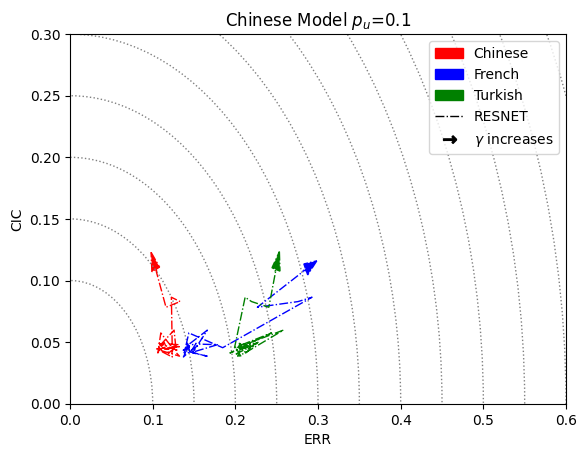
\includegraphics[width=\columnwidth]{Chapter3/FirstPaperFigures/mitigazione_chinese.png}
\caption{Majority - Chin.}
\end{subfigure}
\begin{subfigure}[b]{.325\columnwidth}
\centering
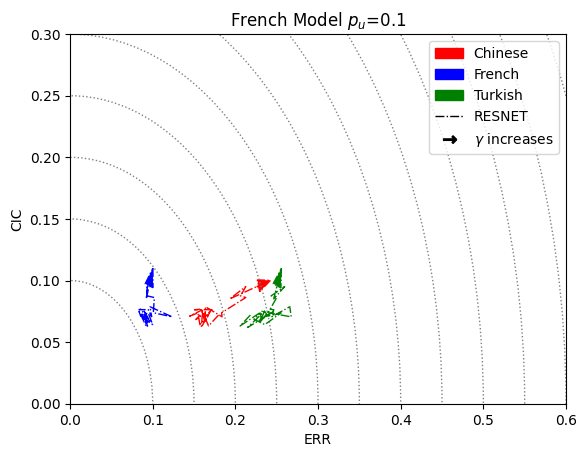
\includegraphics[width=\columnwidth]{Chapter3/FirstPaperFigures/mitigazione_french.png}
\caption{Majority - Fren.}
\end{subfigure}
\begin{subfigure}[b]{.325\columnwidth}
\centering
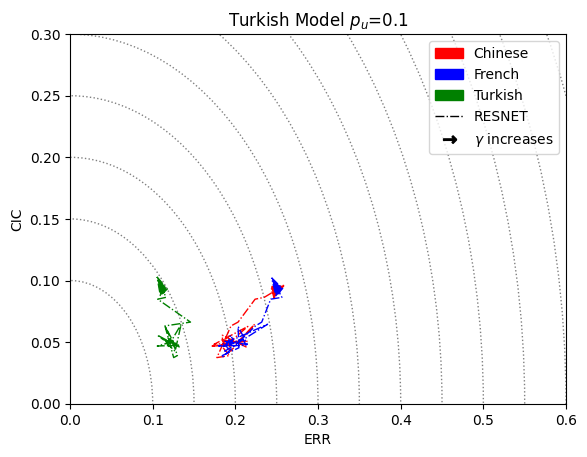
\includegraphics[width=\columnwidth]{Chapter3/FirstPaperFigures/mitigazione_turkish.png}
\caption{Majority - Turk.}
\end{subfigure} 
\caption{LAMP dataset and RESNET algorithm: On the x-axis, we report the average error across all cultures (ERR), while on the y-axis, we report the CIC varying $\gamma$ (with the arrow indicating the direction of increase of $\gamma$), for each combination of majority culture and for each possible combination of the cultures (Chin., Fren, and Turk.) with $p_u = 10\%$.}
\label{ch3:fig:ris:mtl:lamp}
\end{figure}
%
%
\begin{figure}
\centering
\begin{subfigure}[b]{.325\columnwidth}
\centering
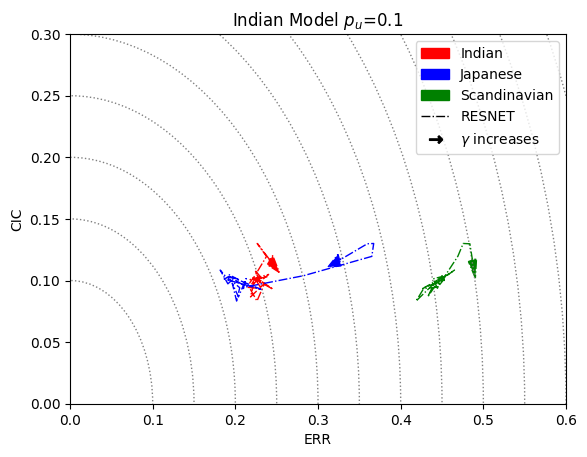
\includegraphics[width=\columnwidth]{Chapter3/FirstPaperFigures/mitigazione_indian.png}
\caption{Majority - Ind.}
\end{subfigure}
\begin{subfigure}[b]{.325\columnwidth}
\centering
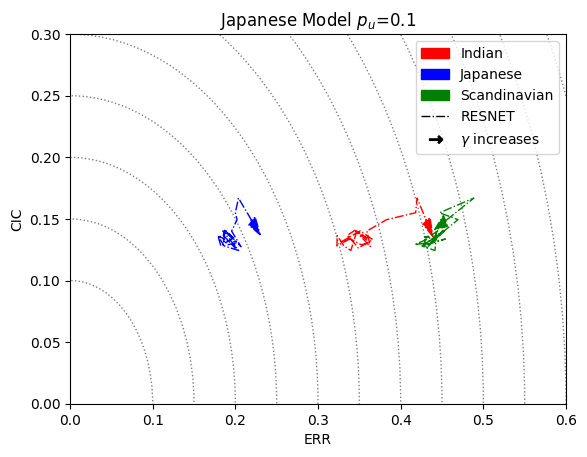
\includegraphics[width=\columnwidth]{Chapter3/FirstPaperFigures/mitigazione_japanese.png}
\caption{Majority - Japan.}
\end{subfigure}
\begin{subfigure}[b]{.325\columnwidth}
\centering
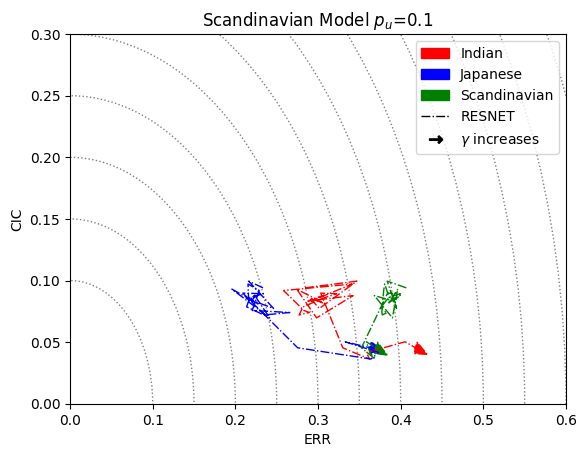
\includegraphics[width=\columnwidth]{Chapter3/FirstPaperFigures/mitigazione_scandianavian.png}
\caption{Majority - Scand.}
\end{subfigure} 
\caption{CARPET dataset and RESNET algorithm: On the x-axis, we report the average error on all cultures (ERR), while on the y-axis, we report the CIC varying $\gamma$ (the arrow indicates the direction of increase of $\gamma$), for each combination of majority culture and each possible combination of the cultures (Ind., Japan., and Scand.) with $p_u = 10\%$.}
\label{ch3:fig:ris:mtl:carpet}
\end{figure}


\section{Conclusion}

This chapter presented a comprehensive empirical evaluation of the cultural competence of standard ML algorithms and the effectiveness of the proposed mitigation strategies across the LAMP and CARPET datasets.

The baseline evaluation demonstrated that standard ML algorithms—LSVM, GSVM, and RESNET—are inherently culturally incompetent under conditions of minority under-representation. Across all majority culture permutations and both datasets, the models consistently exhibited significantly lower error rates for the dominant culture while incurring substantially higher error rates for minority cultures, as quantified by the CIC metric. These disparities persisted even as the minority representation level $p_u$ increased, confirming that cultural incompetence is a structural limitation of standard learning algorithms rather than an artifact of extreme data scarcity.

The MTL-inspired mitigation strategy, applied to the RESNET architecture, demonstrated consistent improvements in both class-specific error rates and CIC across the vast majority of experimental configurations. The task-weighting parameter $\gamma$ proved to be an effective regularization mechanism, enabling the model to balance classification performance with cultural fairness. These results validate the theoretical grounding of the proposed framework and confirm that MTL-based mitigation can be applied effectively across diverse cultural contexts and datasets of varying complexity.

Taken together, these findings establish that standard ML algorithms are not culturally competent by default, and that the proposed MTL-inspired mitigation strategy represents a principled and effective approach to reducing cultural bias in object classification tasks.